\documentclass[10pt, a4paper,spanish]{article}
\usepackage[utf8]{inputenc}

\usepackage{varwidth}
\usepackage{graphicx}

\usepackage[T1]{fontenc} % Use 8-bit encoding that has 256 glyphs
\usepackage{microtype} % Slightly tweak font spacing for aesthetics

\usepackage[hmarginratio=1:1,top=32mm,columnsep=20pt]{geometry} % Document margins
\usepackage[hang, small,labelfont=bf,up,textfont=it,up]{caption} % Custom captions under/above floats in tables or figures
\usepackage{booktabs} % Horizontal rules in tables
\usepackage{float} % Required for tables and figures in the multi-column environment - they need to be placed in specific locations with the [H] (e.g. \begin{table}[H])
\usepackage{hyperref} % For hyperlinks in the PDF

\usepackage{lettrine} % The lettrine is the first enlarged letter at the beginning of the text
\usepackage{paralist} % Used for the compactitem environment which makes bullet points with less space between them

\usepackage{fancyhdr} % Headers and footers
\pagestyle{fancy} % All pages have headers and footers
\fancyhead{} % Blank out the default header
\fancyfoot{} % Blank out the default footer
\fancyhead[C]{ Mayo 2016 $\bullet$ JumpVa $\bullet$ Informe Final} % Custom header text
\fancyfoot[RO,LE]{\thepage} % Custom footer text

%----------------------------------------------------------------------------------------
%	TITLE SECTION
%----------------------------------------------------------------------------------------

\title{\vspace{-15mm}\fontsize{24pt}{10pt}\selectfont\textbf{Informe Final}} % Article title

\author{
\large
\textsc{Sergio García Prado}\\[2mm] % Your name
\normalsize Universidad de Valladolid \\ % Your institution
\vspace{-5mm}
}
\date{\today}

%----------------------------------------------------------------------------------------

\begin{document}
	\begin{titlepage}
	\centering
		%\includegraphics[width=0.15\textwidth]{example-image-1x1}\par\vspace{1cm}
		{\scshape\LARGE Universidad de Valladolid \par}
		\vspace{1cm}
		{\scshape\Large Brooktec S.L.\par}
		\vspace{1.5cm}
		{\huge\bfseries Prácticas en Empresa\par}
		\vspace{2cm}
		{\large
		\textsc{Sergio García Prado\textsubscript}\\[2mm] % Your name
		\vspace{-5mm}
		}

		\vfill

	% Bottom of the page
		{\large \today\par}
	\end{titlepage}

	\thispagestyle{fancy} % All pages have headers and footers

%----------------------------------------------------------------------------------------
%	TABLE OF CONTENTS
%----------------------------------------------------------------------------------------

	\tableofcontents
	\newpage

%----------------------------------------------------------------------------------------
%	TEXT
%----------------------------------------------------------------------------------------



    \section{Datos Generales de la Práctica}



    \section{Breve Descripción de la Empresa}



    \section{Memoria de Actividades}

        \paragraph{}
        Durante mi estancia en la empresa trabajé en varios projectos a la vez que pasé una fase inicial de formación en la cual me familiaricé con las tecnologías que utilizaría más adelante. Las diferentes etapas a veces no están muy bien diferenciadas en la linea temporal ya que hubo proyectos en los que participé al principio y luego se me asignaron otras pequeñas tareas ajenas a ello para después volver a retomar el proyecto.

        \paragraph{}
        Exceptuando la etapa de aprendizaje, en la cual mayoritariamente era yo el encargado de qué hacer (siempre bajo unas guías sobre en qué tecnologías debería adquirir soltura), en el resto de proyectos el patrón de trabajo era el siguiente: Una pequeña explicación acerca de la actividad que debería desempeñar junto con ayuda para configurar el entorno de desarrollo y un conjunto de diseños en los cuales me debía basar para realizar el desarrollo. A partir de este punto mis compañeros me resolvían dudas en el caso de que las tuviera y una vez finalizaba la tarea estos la revisaban antes de subirla al entorno de producción.

        \subsection{Aprendizaje}

            \paragraph{}
            Cronológicamente esta etapa corresponde aproximadamente con las 2 primeras semanas de prácticas, es decir, del 11 al 27 de Julio. Durante esta fase mi labor fue introducirme en el conjunto de herramientas y tecnologías que utiliza Brooktec. Los primeros días me introduje en el lenguaje PHP y mejoré mis conocimientos en JS, HTML y CSS.

            \paragraph{}
            Los primeros días los dediqué a aprender PHP a partir de tutoriales al principio (https://www.codecademy.com/learn/php) y después más en profundidad conociendo frameworks como Slim 3 (microframework para desarrollo de APIs) y Doctrine 2 (librería para mapeo de objetos a un modelo de base de datos relacional). Además de esto y con un entendimiento aceptable de PHP comencé a documentarme sobre el framework de gestión de contenidos WordPress, es decir, para qué sirve, qué facilidades nos aporta, cómo funciona, etc. Para poner en práctica mi aprendizaje con ello cree un tema simple para WordPress y también aprendí a crear plugins, lo cual aporta una gran modularidad a los proyectos basados en ellos.

            \paragraph{}
            A partir de la segunda semana me centré más en el desarrollo Front-end (lo que se ejecuta en el navegador). El lenguaje en el que me basé es TypeScript, cuya característica es que se compila a JavaScript, que es compatible con todos los navegadores. La mayor ventaja de este Lenguaje es que incorpora tipos más estrictos, herencia, interfaces, etc. Además, siguiendo la misma línea, aprendí Less y Sass, cuya utilidad es la misma, pero en este caso aplicada a CSS. También utilicé Bootstrap, un framework que facilita mucho la obtención de resultados muy buenos en el apartado visual de la web. Con todos estos conocimientos empecé a aprender Angular 2, un framework que pretende hacer el desarrollo web mucho más legible y modular. Ya había utilizado anteriormente la primera versión de este framework, pero he de admitir que el cambio ha sido muy grande. Al principio pasé muchos malos ratos hasta que terminé cogiendo el truco a esta nueva manera de verlo, pero he de decir que le terminé cogiendo el gusto y ahora mismo me encanta.

            \paragraph{}
            Para poder desarrollar en todas estas nuevas herramientas también he tenido que utilizar múltiples herramientas. Entre ellas he utilizado Vagrant y Docker, dos entornos de virtualización que me han parecido muy buenas utilidades. También he utilizado Git como herramienta de gestión de versiones (ya lo utilizaba anteriormente con frecuencia pero me ha venido bien para utilizarlo con más soltura.). Para montar un entorno local he utilizado MAMP, el cual configura una pila formada por MySQL, Apache y PHP. Si bien no he tenido que realizar muchos cambios, estos me han venido bien para entender el funcionamiento de Apache e introducirme un poco en SQL y las bases de datos relacionales.

            \paragraph{}
            Por último y para poner en práctica lo que estaba aprendiendo, dediqué los últimos días antes de que me comenzaran a mandar tareas a desarrollar un servicio web para gestionar la lista de la compra. La arquitectura en la que me basé fue la de una API Rest, es decir, un servidor de recursos y una Web App desarrollada en Angular 2 que se comunicaba con el servidor para obtener la información. Estos dos módulos se comunican entre sí mediante ficheros JSON. La ventaja de esta arquitectura es que en el caso de querer ampliar el servicio desarrollando una aplicación móvil, esta utilizaría el mismo servidor de recursos que ya ha sido desarrollado, lo cual ofrece una gran versatilidad.


        \subsection{Nueva Web de SocialNoise}

            \paragraph{}
            Esta nueva etapa comenzó el día 27 de Julio. Fue un gran punto de inflexión ya que a partir de este momento pasé de trabajar en solitario aprendiendo cosas por mi cuenta a trabajar en un equipo de verdad, haciendo cosas por que luego tendrían una mayor transcendencia que el aprender sin más fin que ese. El primer día dediqué la mañana a preparar el entorno de desarrollo (clonando el repositorio, configurando apache, poblando la base de datos, etc).

            \paragraph{}
            El proyecto se basa en la creación desde cero de la nueva web de una empresa dedicada a la publicidad cuyo nombre es SocialNoise. Esta web se apoyaría en WordPress como gestor de contenidos, el cual facilitará la vida a los administradores de la web permitiendoles editar entradas, modificar la plantilla de trabajadores, añadir nuevas muestras de su trabajo, etc. Todo esto sería mucho más complicado para ellos sin este tipo de herramientas.

            \paragraph{}
            Cuando yo empecé a trabajar en este proyecto, este ya llevaba unos días en proceso, por lo cual no pude participar en los primeros momentos. Cuando yo me incorporé lo que había que hacer era desarrollar las  secciones de la nueva web. Trabajé en la parte de Contacto, Ruido (sección de noticias), Clientes, Servicios y colaboré con mis compañeros en  la sección de About. Un apartado muy importante de este trabajo era que para el cliente la versión móvil era muy importante. Toda la página debía seguir el concepto Responsive, adaptando el contenido según el tamaño de la pantalla del dispositivo donde se mostrará.

            \paragraph{}
            Este proyecto me ayudó a entender el funcionamiento de WordPress desde el lado del desarrollador. También aprendí a añadir nuevos tipos de Post con Campos Personalizados. También me dí cuenta del ritmo de trabajo que hay que tener, de que hay que tratar de escribir el código de la manera más legible posible para que otros puedan entender bien lo que has hecho para así poder ampliarlo en un futuro. Una vez que toda la maquetación del sitio web estuvo echa un compañero siguió con ello para centrarse en la parte de animaciones que tendría la página y a mi se me asignaron otras tareas.


        \subsection{Cambios en Webtogo}

            \paragraph{}
            A partir del día 2 de Agosto se me asignaron como tareas un conjunto de cambios en la web de Webtogo. Esta tarea no ha tenido un periodo de tiempo determinado ya que a partir de esta fecha hasta el final de mi periodo de prácticas se me han ido asignando nuevas tareas de modificaciones a realizar cada cierto periodo de tiempo. Dado que la web ya estaba creada y solo eran pequeños cambios en un principio me pareció una tarea fácil y que me llevaría poco tiempo pero más allá de ello, su código daba la sensación de que ya había sufrido otras modificaciones anteriormente, además de que no se habían seguido del todo las guías de estilo al escribir el código.

            \paragraph{}
            Debido a estas carácteristicas tardé más de lo esperado en entender dónde encontrar cada una de las partes de la web que debía modificar. Al cabo de unas horas todos estos problemas fueron redujendose y poco a poco fui entendiendo dónde estaban las partes que tenía que modificar. Los primero cambios que se me asignaron fueron unas imágenes en la página principal, modificaciones en las cabeceras de todas las secciones y de un submenu que aparece en las mismas. Fue en estos cambios donde empecé a hacer mis propias consultas personalizadas a WordPress (para encontrar relaciones entre secciones y subsecciones por ejemplo).

            \paragraph{}
            La segunda fase de tareas de esta web que se me asignaron comenzó el 22 de Agosto. Este era otro conjunto de cambios para dicha web la cual se basaba en cambios de estilos como colores y tamaños a partir del CSS, añadir animaciones en la barra superior al hacer scroll, solucionar un problema que había al importar fuentes desde otras url externas, corregir fallos al visualizar la versión móvil, etc. Con estos cambios ya no tuve tantos problemas como con los primeros porque ya conocía mejor cómo estaba organizada la web.


        \subsection{Nueva sección Descubre ERL de El Rey León}

            \paragraph{}
            Este proyecto se me asignó el 8 de agosto y trabajé en el durante el resto del mes, primero como tarea principal y durante la ultima semana a través de tareas de feedback que proponía el cliente. Esta tarea consistió en la colaboración en el desarrollo de una nueva sección en la web del Musical El Rey León. Esta sección se denominaría Descubre El Rey León y estaría destinada en acercar el musical a la gente para que así vayan más personas a ver la obra.

            \paragraph{}
            Cuando yo me incorporé a este proyecto, este ya había sido empezado, estando ya desarrollada toda la parte visual del mismo, por lo que lo que quedaba era implementar la funcionalidad. Esta nueva sección estaba formada por dos galerías  de imágenes animadas, un reproductor musical que obtiene los recursos a partir de SoundCloud en el cual se puede votar cual es la canción que más te gusta, una votación sobre cuál es el personaje que más te gusta y por último un tweet destacado.

            \paragraph{}
            Para implementar la funcionalidad decidí modularizar los componentes como plugins para que así fuera más simple su migración a otras webs. Los dos tipos de votaciones almacenan los resultados en la propia base de datos de wordpress habiendo creado tablas personalizadas para dicha utilidad. En el caso del plugin de reproductor con votaciones se ha desarrollado mayoritariamente en JS con ayuda de jQuery debido a que las canciones se obtienen a partir de un servidor externo y no tiene sentido desarrollarlo en PHP (lado del servicdor).

            \paragraph{}
            Fue trabajando en esta tarea donde empecé a hacer animaciones sencillas por mi cuenta, que a pesar de ser simples me sirvieron como una introducción. Este fue un requisito impuesto por el cliente para esta nueva sección. También mejoré mis conocimientos en JS y jQuery, ya que no la había utilizado en profundidad hasta ese momento. Una vez más, trabajé algo con bases de datos relacionales, lo cual me sirvió para aprender conceptos básicos que debido a que todavía no he cursado la corresponiente asignatura en la Universidad, todavía no tengo.


        \subsection{Nueva Web de Legal Lifeline}

            \paragraph{}
            A este proyecto me incorporé el día 24 de Agosto. La principal característica de él es que estaba en una base muy inicial, es decir, tan solo estaba creada la estructura, por lo cual me sirvió para conocer las primeras fases de desarrollo de una web con WordPress. La otra gran característica de este proyecto es su manera de ejecución. El entorno está construido a partir de Docker, una tecnología poco conocida para mí hasta ese momento pero que me sirvió de gran ayuda para conocerla. A pesar de tardar un día entero para tener todo el entorno de desarrollo montado (ya que tuve que realizar algunos tutoriales para conocer su funcionamiento).

            \paragraph{}
            Una vez que tenía todo listo empecé a desarrollar la sección de testimos, caracterizada por pertenecer a determinadas categorías. Para ello tuve que crear un nuevo tipo de post así como una categoría. Estos se muestran en la en forma de grid de categorias y al clickar sobre una de ellas se habre un modal (ventana emergente) que contiene todos los testimonios.

            \paragraph{}
            La otra sección que desarrollé para este proyecto era la página de ayuda, la cual tiene unas preguntas ya contestadas por los administradores de la web y permite la posibilidad de buscar preguntas con la intención de encontrar alguna que se asemeje a la duda que se tenga. En el caso de que no se encontrase se permite preguntar esta duda para que los administradores puedan contestarla.
            

    \section{Conclusiones}



    \newpage
    \section{Declaración de Responsabilidad}

        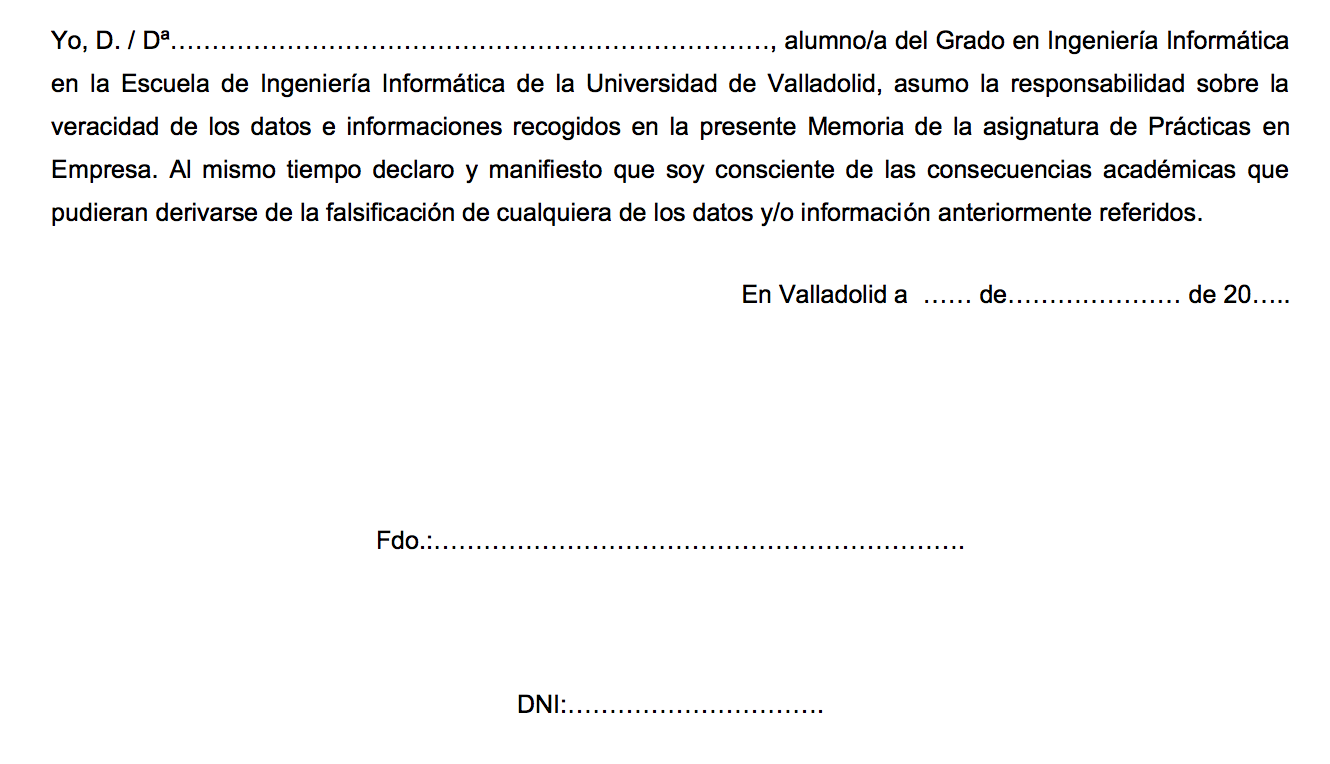
\includegraphics[width=\textwidth]{res/responsibility-declaration}



\end{document}
